\documentclass{article}

\usepackage[utf8]{inputenc}
\usepackage{amsmath}
\usepackage{amsfonts}
\usepackage{bbold}
\usepackage{bm}
\usepackage{graphicx}
\usepackage{booktabs}
\usepackage[backend=bibtex]{biblatex}

\addbibresource{references.bib}

\newcommand*{\todo}[1]{\footnote{\textbf{TODO:} {#1}}}
\newcommand*{\etal}[1]{\textit{et al.}}

% special letters denoting sets and algebras
\providecommand*{\Nset}{\mathbb{N}}  % naturals
\providecommand*{\Qset}{\mathbb{Q}}  % rationals
\providecommand*{\Zset}{\mathbb{Z}}  % integers
\providecommand*{\Rset}{\mathbb{R}}  % reals

% calligraphic alphabet
\newcommand*{\calA}{\ensuremath{\mathcal{A}}}
\newcommand*{\calB}{\ensuremath{\mathcal{B}}}
\newcommand*{\calC}{\ensuremath{\mathcal{C}}}
\newcommand*{\calD}{\ensuremath{\mathcal{D}}}
\newcommand*{\calE}{\ensuremath{\mathcal{E}}}
\newcommand*{\calF}{\ensuremath{\mathcal{F}}}
\newcommand*{\calG}{\ensuremath{\mathcal{G}}}
\newcommand*{\calH}{\ensuremath{\mathcal{H}}}
\newcommand*{\calI}{\ensuremath{\mathcal{I}}}
\newcommand*{\calJ}{\ensuremath{\mathcal{J}}}
\newcommand*{\calK}{\ensuremath{\mathcal{K}}}
\newcommand*{\calL}{\ensuremath{\mathcal{L}}}
\newcommand*{\calM}{\ensuremath{\mathcal{M}}}
\newcommand*{\calN}{\ensuremath{\mathcal{N}}}
\newcommand*{\calO}{\ensuremath{\mathcal{O}}}
\newcommand*{\calP}{\ensuremath{\mathcal{P}}}
\newcommand*{\calQ}{\ensuremath{\mathcal{Q}}}
\newcommand*{\calR}{\ensuremath{\mathcal{R}}}
\newcommand*{\calS}{\ensuremath{\mathcal{S}}}
\newcommand*{\calT}{\ensuremath{\mathcal{T}}}
\newcommand*{\calU}{\ensuremath{\mathcal{U}}}
\newcommand*{\calV}{\ensuremath{\mathcal{V}}}
\newcommand*{\calW}{\ensuremath{\mathcal{W}}}
\newcommand*{\calX}{\ensuremath{\mathcal{X}}}
\newcommand*{\calY}{\ensuremath{\mathcal{Y}}}
\newcommand*{\calZ}{\ensuremath{\mathcal{Z}}}

% bold letters
\newcommand*{\veca}{\bm{a}}
\newcommand*{\vecb}{\bm{b}}

% functions
\newcommand*{\One}{\mathbb{1}}
\newcommand*{\normtwo}[1]{\| #1 \|}

% set theory
\newcommand*{\union}{\cup}
\newcommand*{\inters}{\cap}
\newcommand*{\setdiff}{\setminus}

% topics commands
\newcommand*{\cls}{\text{cls}}
\newcommand*{\attr}{\text{attr}}
\newcommand*{\iou}{\text{IoU}}
\newcommand*{\bbox}{\bm{b}}
\newcommand*{\qj}{\bm{q}_j}
\newcommand*{\eqj}{e^{\qj}}
\newcommand*{\Eqj}{E^{\qj}}
\newcommand*{\ePI}{e^{\calP_{\bm{I}}}}
\newcommand*{\EPI}{E^{\calP_{\bm{I}}}}
\newcommand*{\fsim}{f_{\text{sim}}}
\newcommand*{\fagg}{f_{\text{aggregate}}}
\newcommand*{\fapplysim}{f_{\text{apply sim}}}
\newcommand*{\floss}{f_{\text{loss}}}
\newcommand*{\fdir}{f_{\text{dir}}}

\title{Unsupervised Visual-Textual Grounding based on Concept Similarity}
\author{Luca Parolari}
\date{November 2021}

\begin{document}

\maketitle

\section{Introduction}

In this work we propose a simple and interpretable model that learns
from concept similarity. The goal is to solve phrase localization
problem under unsupervised settings. Given a noun phrase, we define
it's concept as the most important word in the phrase, while, given a
bounding box we define it's class as the label, among a dictionary of
labels, predicted by an object detector for that bounding box. The
concept similarity is the similarity between the phrase concept and
bounding box class. Here, the key idea is that the head of the phrase
should be very similar (semantically speaking) to the content of the
bounding box and thus, to its class. Indeed, we optimize the model to
learn a representation where similar concepts from image and text
should be close each other, otherwise they are forced to be
perpendicular. The model is unsupervised because no ground truth is
used during training and supervision is enforced throught a similarity
function computed among concepts.

% Our model is straightforward. First of all, we gather image features
% from the object detector and we compute five additional features
% representing bounding box top left and bottom right corners and area
% (spatial features). We then project those features to a subspace,
% performing a dimensionality reduction. Regarding the text, we fisrt
% compute the word embeddings using a pretrained word emebdding and then
% we encode the phrase throught an LSTM recurrent neural network. Our
% predictions are the results of the cosine similarity between projected
% image features and the last LSTM hidden neuron. In order to obtain the
% weak supervision, we compute concept similarity which is required to
% weakly supervise learning by attracting or repulsing features. The
% attraction is performed when concept similarity between two modalities
% is above a given threshold, otherwise repulsion is applied. Moreover,
% we accompany to concept similarity the attribute similarity which
% helps discriminate between same class bounding boxes. 

\section{Background}

\subsection{Phrase Localization}

Given in input an image $\bm{I}$ and a
sentence $\mathrm{S}$, phrase grounding consists in learning a mapping
$\gamma$ from the set $\calQ$ of noun phrases to a set of bounding box
$\calB$ defined on $\bm{I}$, i.e., $\gamma : \calI \times \calS
\rightarrow 2^{\calQ \times \calB}$ \cite{rigoni2021better}. So, given
an image $\bm{I}$ containing $e$ objects identified via the set of
bounding boxes $B_\calI = \{ b_i \}^e_{i=1}$, where $b_i \in \Rset^4$
is the vector of coordinates identifying a bounding box in $\bm{I}$,
and a sentence $\mathrm{S}$ containing $m$ noun phrases gathered in
the set $\calQ_S = \{ q_j \}^m_{j=1}$, where $q_j \in \Nset^2$ is a
vector containing as coordinates the initial and final character
positions in the sentence $\mathrm{S}$, $\gamma(\bm{I}, \mathrm{S})$
returns a set of couples $\{ (\bm{q}, \bm{b}) \mid \bm{q} \in
\calQ_{\mathrm{S}}, \bm{b} \in B_{\bm{I}} \}$ where each couple
$(\bm{q}, \bm{b})$ associates the noun phrase $\bm{q}$ to the bounding
box $\bm{b}$. Please, notice that the same noun phrase can be
associated to several different bounding boxes, as well as the same
bounding box can be associated to many different noun phrases.
Following the current literature, we assume that each noun phrase is
associated to one and only one bounding box. Bounding boxes, however,
can identify more objects, e.g. several persons in the case the noun
phrase is ``people''.

\section{Model}

In the following sections we describe the model architecture, outlined
in Fig.\ref{fig:model-architecture}.

\begin{figure}
    \centering
    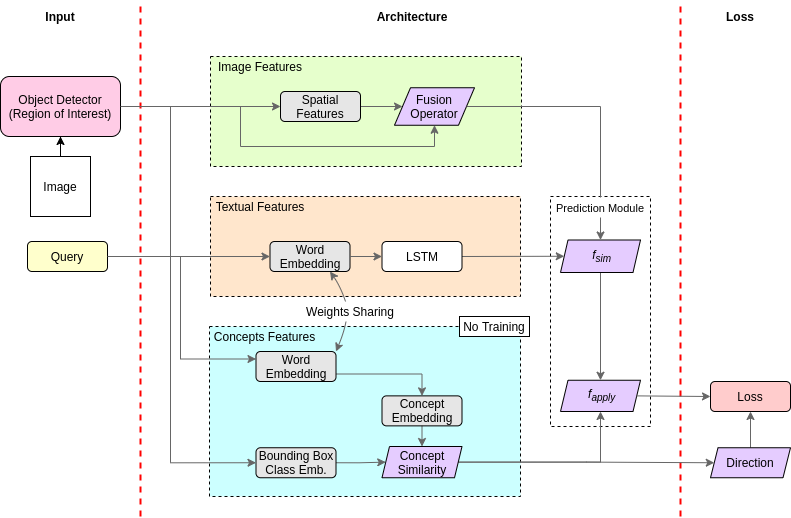
\includegraphics[width=1.0\textwidth]{figures/model-architecture.png}
    \caption[TODO]{Our model architecture overview. [WORK IN PROGRESS]}
    \label{fig:model-architecture}
  \end{figure}

\subsection{Visual Branch}

Given an image $\bm{I}$, we extract a set of $k$ bounding box
proposals $\calP_{\bm{I}} = \{ \bm{p}_i \}^k_{i=1}$ by means of a
pre-trained object detector, where $p_i \in \Rset^4$, jointly with
features $H^v = \{ \bm{h}^v_i \}^k_{i=1}$, where $\bm{h}^v_i \in
\Rset^v$. The features represent the internal object detector
activation values before the classification layers and regression
layer for bounding boxes. Moreover, our model extracts the spatial
features $H^s = \{ \bm{h}^s_i \}^k_{i=1}$, where $\bm{h}^s_i \in
\Rset^s$ from all the bounding boxes proposals, with the spatial
features for the proposal $\bm{p}_i$ defined as:
\begin{equation}
  \bm{h}^s_i = \left[ \frac{x1}{wt}, \frac{y1}{ht}, \frac{x2}{wt}, \frac{y2}{ht}, \frac{(x2 - x1) \times (y2 - y1)}{wt \times ht}  \right]
\end{equation}
where $(x1, y1)$ refers to the top-left bounding box corner, $(x2,
y2)$ refers to the bottom-right bounding box corner, $wt$ and $ht$ are
the width and height of the image, respectively. Both visual and
spatial features are then concatenated, thus leading to a set of new
vectorial representations $H^{||} = \{ \bm{h}^{||}_{jz} \}_{j \in [1,
\ldots, m], z \in [1, \ldots, k]}$, where vectors $\bm{h}^{||}_{jz}$
are defined as:
\begin{equation}
  \bm{h}^{||}_{jz} = \Big( \bm{W}^{||} \left( \bm{h}^s_z || L1(\bm{h}^v_z) \right) + \bm{b}^{||} \Big) 
\end{equation}
where $||$ indicates the concatenation operator, $\bm{h}^{||}_{jz} \in
\Rset^c$, $\bm{W}^{||} \in \Rset^{c \times (s + v)}$ is a matrix
of weights, $\bm{b}^{||} \in \Rset^c$ is a bias vector, and $L1$ is
the L$1$ normalization function.

% We also assume that the object detector returns, for each $\bm{p}_i$,
% a probability distribution $Pr_{Cls}(\bm{p}_i)$ over a set $Cls$ of
% predefined classes, i.e. the probability for each class $\zeta \in
% Cls$ that the content of the bounding box $\bm{p}_i$ belongs to
% $\zeta$. This information is typically returned by most of the object
% detectors, and it will be used to define our novel loss function.
% \todo{UPDATE: to define our...}

\subsection{Textual Branch}

Regarding the textual features extraction, given a noun phrase
$\bm{q}_j$, initially all its words $W^{\bm{q}_j} = \{ w^{\bm{q}_j}_i
\}^l_{i=1}$ are embedded in a set of vectors $E^{\bm{q}_j} =
\{e^{\bm{q}_j}_i \}^l_{i=1}$ where $e^{\bm{q}_j}_i \in \Rset^w$, where
$w$ is the size of the embedding. Then, our model applies a LSTM
neural network to generate from the sequence of word embeddings only
one new embedding $\bm{h}^*_j$ for each phrase $\bm{q}_j$. This
textual features extraction is defined as:
\begin{equation}
  \bm{h}^*_j = L1(LSTM(E^{\bm{q}_j}))
\end{equation}
where $\bm{h}^*_j \in \Rset^t$ is the LSTM output of the last word in
the noun phrase $\bm{q}_j$, and $L1$ is the L$1$ normalization
function.

\subsection{Similarity Branch}

Along with visual and textual features we also compute a similarity
score between noun phrases and bounding box class labels, the concept
similarity \cite{wang2019phrase}. The similarity score is computed
between pretrained embeddings, i.e., feature vectors, where each on
represents a word from a dictionary and hopefully captures semantic as
well as syntactic information.

Formally, we define $\EPI = \{\ePI_i \}^{k}_{i=1}$ the set of class
labels embeddings build on the set of proposal $\calP^{\bm{I}}$. Each
$\ePI_i$ is a feature vector representing the class label predicted
with maximum confidence by the object detector for the $i$-th
proposal. Then, given a noun phrase $\bm{q}_j$ along with
$E^{\bm{q}_j}$, we compute the concept similarity score for each
proposal $i$ and phrase $j$ as:
\begin{equation}
  \bm{S}^c_{ji} = \fsim \left( \xi_j, \ePI_i \right),
\end{equation}
where $\fsim$ is a similarity measure such us the cosine similarity,
and $\xi$ is the embedding representing the concept of the noun phrase
$\qj$:
\begin{equation}
  \xi_j = \fagg(\Eqj, \EPI).
\end{equation}
The new embedding $\xi_j$ can be computed with different strategies: for
example, we can simply compute the mean of all word embeddings in the
noun phrase:
\begin{equation}
  \fagg^{\text{mean}}(\Eqj, \EPI) = \frac{\sum^l_{i=1} \eqj_i}{| \Eqj |},
\end{equation}
or use only the last word as done in \cite{wang2019phrase}:
\begin{equation}
  \fagg^{\text{last}}(\Eqj, \EPI) = \eqj_l.
\end{equation}
More complex strategies, instead, take into account external
information, such us the similarity wrt proposal class embeddings.
Here, we compute the similarity between word in noun phrase and
proposal class embeddings and then we select one word in the noun
phrase with maximum similarity wrt the detected concept in proposal:
\begin{equation}
  \fagg^{\text{max}}(\Eqj, \EPI) = \max_{\eqj \in \Eqj} \{ \max g(\eqj) \},
\end{equation}
where
\begin{equation}
  g(\eqj) = \{ \fsim(\ePI, \eqj) \mid \ePI \in \EPI \}.
\end{equation}

\subsection{Prediction Module}

Finally, the model predicts the probability $\bm{P}_{jz}$ that a given
noun phrase $\qj$ is referrred to a proposal bounding box $\bm{p}_z$
as:
\begin{equation}
  \bm{P}_{jz} = \fsim ( \bm{h}^{||}_{jz} , \bm{h}^*_j ).
\end{equation}

As noted in \cite{chen2018knowledge}, concept similarity is a direct
consequence of the intrinsic knwoledge convoyed by the object
detector. Such score can be useful to down-weight unrelated proposals.
Its effectiveness is due to the fact that the word embedding usually
captures the semantic similarity between concept in phrase and the
content of the bounding box, and thus, let the model focuses on
relevant proposals. Thus, a straightforward improvement to our base
model would be to include this knowledge and exploit it for making
predictions. Hence, we can apply the concept similarity on previously
computed predictions $\bm{P}_{jz}$ as:
\begin{equation}
  \bm{\hat{P}}_{jz} = \fapplysim \left( \bm{S}^c_{jz}, \bm{P}_{jz} \right).
\end{equation}

The simplest strategy for applying the concept similarity to
previously computed predictions is by multiplying the two, treating
$\bm{S}^c_{jz}$ as a weight matrix:
\begin{equation}
  \fapplysim^{\text{prod}} (\bm{S}^c_{jz}, \bm{P}_{jz}) = \bm{S}^c_{jz} * \bm{P}_{jz}.
\end{equation}
At first glance, this approach seems very promising because we force
the model to return predictions ``on steroid'' when there is a
semantic relation between phrase and proposal or downweighted when no
similarity is found. However, this relies on the assumption that the
embedding space and similarity measure we are using for words
perfectly captures the semantic similarity between them, and this is
not true. Also, we assume that proposals are classified with no error
by the object detector, neither this is true. Under those hypotesis,
such application of concept similarity cannot be fruitful. 

A more convenient way of applying concept similarity to prediction is
instead to compute the mean between two. Eventually, we can also put a
weight $\lambda$ with values in $[0 .. 1]$ in order to balance
contributions. Formally, $\fapplysim$ becomes:
\begin{equation}
  \fapplysim^{\text{mean}} (\bm{S}^c_{jz}, \bm{P}_{jz}) = (1 - \lambda) * \bm{S}^c_{jz} + \lambda * \bm{P}_{jz}.
\end{equation}
The major benefit of this approach is that model predictions are not
constrained to values defined by concept similarity.

\section{Training}

In this section we present our loss function. For the sake of
presentation, we define in the following the loss terms referred to a
single example. The total loss is then obtained by summing up the
contributions of all examples in the training set.

Please note that in unsupervised settings, for a training example
$\left( \bm{I}, S \right)$ we are not given the query-proposal pair
set $\{ ( q^{gt}_j, p^{gt}_j ) \}^m_{j=1}$, where $m$ is the number of
noun phrases. To tackle this problem, in our work we adopt a very
simple strategy: we exploit concept similarity. Basically, we attract
representations whose concept similarity is above a certain treshold,
otherwise we want to repulse them. We define our oracle as:
\begin{equation}
  \bm{D}_{jz} =
  \begin{cases}
    1, & \bm{S}^c_{jz} > \alpha \\
    -1, & \text{otherwise}
  \end{cases},
\end{equation}
where $\bm{S}^c$ is the concept similarity matrix, $j$ is the
$\alpha$ is the threshold. This policy relies on the assumption that
concept similarity correctly captures the semantic relation between
query and proposal. $\bm{D}$ is the concept direction matrix.

Now, given a training example $\left( \bm{I}, S \right)$, where
$\cal{P}_{\bm{I}}$ the bounding box proposals set, we define the loss
function $\calL$ (for a single example) as:
\begin{equation}
  \calL = \frac{1}{m} \sum^m_{j=1} \Bigg( \frac{1}{z} \sum^k_{z=1} \floss ( \bm{P}_{jz}, \bm{D}_{jz} ) \Bigg)
\end{equation}
where $m$ in the number of noun phrases, $k$ is the number of proposal
bounding box, $\bm{P}_{jz}$ is the model predicted probability that
the noun phrase $\bm{q}_j \in \calQ$ refers to the image content
localized by $\bm{p}_z \in \calP_{\bm{I}}$. Our loss is scaled by $m$
and $k$ because number of noun phrase can change, but also number of
proposal. 

We optimize the model to learn features representation in the
similarity space, such that the depiction of $\bm{p}_z$ and $\bm{q}_j$
are neighbors when $\bm{D}_{jz}$ is $1$, perpendicular otherwise.
Formally:
\begin{equation}
  \floss^{\text{orthogonal}} \left( \bm{P}_{jz}, \bm{D}_{jz} \right) = - \bm{D}_{jz} \bm{P}^+_{jz} + \left( \bm{D}_{jz} \bm{P}^-_{jz} \right)^2,
\end{equation}
where $\bm{P}^+_{jz} = \One\left( \bm{D}_{jz} \right) \bm{P}_{jz}$
is the matrix that keeps predictions whose concept direction is over
the threshold and cancel the other, $\bm{P}^-_{jz} = \One\left( -
\bm{D}_{jz} \right) \bm{P}_{jz}$ instead cancels prediction with
concept similarity above threshold; $\One$ is the unit step function
\begin{equation}
  \One(x) =
  \begin{cases}
    1, & x \geq 0 \\
    0, & \text{otherwise}
  \end{cases}.
\end{equation}

Also in this case, some different strategies are available. Instead of
optimizing repulsed features to be perpendicular, one could also
exploit the similarity space and force them to be inversely
correlated. Another improvement would be to normalize the score by
number of bounding box with same class label. Indeed, due to the
long-tail distribution of bounding box class labels in dataset, some
representations are moved more than other: the normalization allows to
introduce a kind of equality.

\section{Experiment and Results}

Experiments were carried out on Flickr30k Entities and ReferIt dataset
using common train, valid, test split sets made availabe by dataset
authors. Results are evaluated thought standard accuracy, where a
predicted bounding box $\bm{p}_z$ for a query phrase $\bm{q}_j$ is
considered correct if its intersection over union (IoU) with the
ground truth $\bm{p}^{gt}_z$ is at least 50\%, and poiting game
accuracy, where an hit is considerect correct whether the center of
the predicted bounding box $\bm{p}_z$ falls inside the ground truth
bounding box $\bm{p}^{gt}_z$.

The Tab.~\ref{tab:results} shows performance comparison on Flickr30k
Entities dataset.\footnote{For time reasons, we are concentrating our
efforts on Flickr30k Entities. Here, we do not report ReferIt results
because we still have to run last experiments on it and we already
outperformed all SotA works.} We outperformed by $5$\% best previous
SotA work with pointing game accuracy. With standard accuracy instead
we obtain nearly $6$\% worse results compared to
\cite{wang2019phrase}, outperforming all other works. In
\cite{wang2019phrase}, they do not train a model: they use many
pretrained object detectors in order to semantically match the content
of the proposal with the concept of the phrase, then they disambiguate
the between candidate proposals with a fixes strategy. We argue that,
even if this is an intereseting approach, it higly depends on how a
dataset is built. (For example, we outperform their model by $8$\%
accuracy on ReferIt). Flick30k Entities is an high-quality dataset,
but it is not exempt to some problems, such us the long-tail
distribution on bounding box class labels. A model without a training
stage is bound to leverage on the statistical distribution of data
wihtout any possible improvement.

\begin{table}
  \centering
  \bgroup
  %\def\arraystretch{1.5}
  \resizebox{\textwidth}{!} {%
  \begin{tabular}{lccc}
    \toprule
    \textbf{Approach} & \textbf{Supervision} & \textbf{Acc. (\%)} & \textbf{P. Acc. (\%)} \\
    \midrule
    Top-Down Visual Saliency \cite{ramanishka2017top}        & weak & -    & 50.1 \\
    KAC Net \cite{chen2018knowledge}                         & weak & 37.7 & -    \\
    Semantic Self-Supervision \cite{javed2018learning}       & weak & -    & 49.1 \\
    Multi-level Multimodal \cite{akbari2019multi}            & weak & -    & 57.9 \\
    Align2Ground \cite{datta2019align2ground}                & weak & 11.5 & 71.0 \\
    Localziation w/o Training Examples \cite{wang2019phrase} & no   & \textbf{50.5} & -    \\
    Grounding By Separation \cite{arbelle2021detector}       & weak & -    & 70.5 \\
    \midrule
    Ours                                                     & no   & 43.9 & \textbf{75.5} \\
    \bottomrule
  \end{tabular}
  }
  \egroup
  \caption{
    Performace comparison on Flickr30k Entities dataset. \textit{Acc.}
    is the standard accuracy, while \textit{P. Acc.} is the poiting
    game accuracy. (Greater is better). Values in bolds represent best
    performance. Works are listed by publication date.
  }
  \label{tab:results}
\end{table}

\pagebreak
\printbibliography

\end{document}
